% ============================================
%  Article Class (This is a LaTeX2e document)
% ============================================
\documentclass[12pt]{scrartcl}
\usepackage[english]{babel}
\usepackage[round]{natbib}
\usepackage[T1]{fontenc}
\usepackage{color}

% ============================
%  Figures and relative paths
% ============================
\usepackage{graphicx}
\graphicspath{{figures/}}

% =======================
%  References to classes
% =======================
\usepackage[colorlinks=true]{hyperref}
\newcommand{\rbametabolism}{\hyperref[sec:rba_metabolism]{\textbf{RBAMetabolism}}}
\newcommand{\compartment}{\hyperref[sec:compartment]{\textbf{Compartment}}}
\newcommand{\species}{\hyperref[sec:species]{\textbf{Species}}}

% ==========
%  Document
% ==========
\begin{document}

\title{XML format for RBA models}
\author{S. Fischer, V. Fromion, A. Goelzer}
\date{\today}

\maketitle

\newpage

\tableofcontents

\newpage

\section{Introduction}

In this document we present the XML structures used to define a RBA model.
A complete RBA model is composed of the following files:
\begin{itemize}
  \item metabolism.xml
  (definition of compartments, metabolic species and metabolic reactions).
  \item parameters.xml
  (definition of density constraints and user-defined functions).
  \item proteins.xml (definition of proteins).
  \item rnas.xml (definition of RNAs).
  \item dna.xml (definition of DNA).
  \item enzymes.xml
  (definition of enzymatic machineries catalyzing metabolic reactions).
  \item processes.xml
  (definition of cell processes necessary to growth and maintenance).
\end{itemize}

For every file, we present the nodes that composes the XML structure.
For every node, we show a class diagram that shows the node's attributes
and the children node that it may/must contain.
We provide a brief description about the relevance of the node
in the RBA model.


\section{Conventions}

\subsection{Naming conventions}

\subsection{Boolean attributes}


\section{metabolism.xml}

The metabolism file is strongly inspired by SBML.\@
More precisely, it can be seen as a subpart of an SBML file.
It is used to define compartments, metabolites and reactions.

\subsection{Rationale}

metabolism.xml contains the most basic bricks of an RBA model.
In our effort to define a minimal structure that contains an RBA model,
we decided to start with an SBML structure and strip it down to elements that
are essential to RBA.

metabolism.xml defines the structure of the metabolic network:
simple chemical species (metabolites) that flow between compartments through
transport reactions or transformed into other simple chemical species that
will be available as building blocks for more complex molecules.

The description is entirely static: input fluxes are defined
through the medium and parameters.xml, output fluxes are
defined by targets.xml, the dynamics of internal fluxes is
defined in enzymes.xml.

\subsection{RBAMetabolism}
\label{sec:rba_metabolism}

The outermost part of the metabolism file is an instance of class
\rbametabolism, shown in Figure~\ref{fig:metabolism_doc}.

\begin{figure}
  \centering
  \includegraphics[scale=0.8]{figures/metabolism_doc}
  \caption{XML structure of metabolism document.}
\label{fig:metabolism_doc}
\end{figure}

Currently, \rbametabolism{} has no simple attributes.
It includes exactly one instance of each \textbf{ListOf} container class.
All \textbf{ListOf} classes do not have own attributes,
they are merely used to organize a list of instances from another class.
This organization was inspired by SBML.\@


\subsection{Compartment}
\label{sec:compartment}

The \compartment{} class is used to list existing cell compartments.

\paragraph{The \textit{id} attribute}
The \textbf{id} attribute is a string defining the identifier of a compartment.
Every compartment should have a different id.


\subsection{Species}
\label{sec:species}

The \species{} class is used to define \emph{metabolic} species.

\paragraph{The \textit{id} attribute}
The \textbf{id} attribute is a string defining the identifier of a metabolite.

\paragraph{The \textit{boundaryCondition} attribute}
The \textbf{boundaryCondition} attribute is a boolean.
If the attribute is set to true, the metabolite is considered to be at
a constant concentration.
In other words, it is not affected by reactions.
This is typical for metabolites in the external medium.


\subsection{Reaction}
\label{sec:reaction}

The \reaction{} class is used to define metabolic reactions
(Fig.~\ref{fig:metabolism_reaction}).
Reactants and products are defined using a \textbf{ListOfSpeciesReferences}.

\begin{figure}
  \centering
  \includegraphics[scale=0.8]{figures/metabolism_reaction}
  \caption{Class storing metabolic reactions.}
\label{fig:metabolism_reaction}
\end{figure}

\paragraph{The \textit{id} attribute}
The \textbf{id} attribute is a string defining the identifier of a reaction.

\paragraph{The \textit{reversible} attribute}
The \textbf{reversible} attribute is a boolean.
If the attribute is set to true, the reaction can occur in both directions.
If the attribute is set to false, only the forward reaction can occur.


\subsection{SpeciesReference}
\label{sec:species_reference}

The \speciesreference{} class is used to refer to a metabolic \species{}
and associate with it a stoichiometry (Fig.~\ref{fig:metabolism_reaction}).

\paragraph{The \textit{species} attribute}
The \textbf{species} attribute must match the identifier of a \species{}.

\paragraph{The \textit{stoichiometry} attribute}
The \textbf{stoichiometry} is a positive real number.
It repensents the stoichiometry of a \species{} in a given context
(typically a \reaction).

\subsection{Examples}

Figure~\ref{fig:metabolism_ex_1} shows a very simple example with 2 compartments,
4 metabolites and 3 reactions.
In this example, we tagged \texttt{M\_carbon\_source\_e} with \texttt{boundary\_condition="true"},
implying that it is an external metabolite whose concentration is known and set through the
medium in medium.tsv.
Boundary metabolites are essential in the model, as they define input fluxes in the model.

\begin{figure}
  \includegraphics[scale=0.6]{figures/metabolism_ex_1}
  \caption{metabolism.xml from the minimal model with 2 compartments,
  4 metabolites and 3 reactions.}
\label{fig:metabolism_ex_1}
\end{figure}

Note that the description of the metabolic network ends with the protein precursor.
Proteins \emph{should not} be defined in metabolism.xml.
Their composition is described in proteins.xml, while their assembly is described in processes.xml.


\section{parameters.xml}

The parameter file contains user-defined parameters and functions.

\subsection{Rationale}

The file parameters.xml contains all numerical values occurring in the model
(except for stoichiometries).
Nearly all other files refer to this file, as we have seen throughout the
examples, where numerical values were defined as parameter identifiers.
The most common parameters are: total amino acid concentrations,
fractions of protein per compartment,
percentages of non-enzymatic protein per compartment and cellular machinery,
target fluxes for metabolites and macromolecules, efficiencies of enzymes,
transporters and molecular machines.

A parameter may be defined as: a constant, a function of growth rate,
or a function of an external metabolite concentrations (defined in medium.tsv).
Currently, the format supports the following function types:
linear, inverse, exponential and Michaelis-Menten.
The function types have been chosen to reflect common biochemical functions.
Typically, enzyme efficiencies vary linearly with growth rate
and transporters have activities that depend on the concentration of metabolites transported
according to a Michaelis-Menten function.

A parameter can also be defined as a product of functions, called an “aggregate”.
For example, the activity of a transporter can be described
as the product of a growth rate-dependent maximal activity and a
concentration-dependent Michaelis-Menten term.
All parameters are allowed to have growth-rate or concentration dependencies.
For instance, maximal densities and target fluxes can be defined as constant or growth rate dependent.

\subsection{RBAParameters}
\label{sec:rba_parameters}

The outermost part of the parameter file is an instance of class
\rbaparameters, shown in Figure~\ref{fig:parameters_doc}.

\begin{figure}
  \centering
  \includegraphics[scale=0.8]{figures/parameters_doc}
  \caption{XML structure of parameter document.}
\label{fig:parameters_doc}
\end{figure}

\rbaparameters{} has no simple attributes.
It includes exactly one instance of \textbf{ListOf} container classes.
All \textbf{ListOf} classes do not have own attributes,
they are merely used to organize a list of instances from another class.

\subsection{Function}
\label{sec:function}

The \function{} class is used for user-defined functions and parameters
(Fig.~\ref{fig:parameters_function}).
The default variable of a function is the growth rate, but it may also be
the extracellular concentration of a metabolite.
Every function holds a \textbf{ListOfParameters},
where \parameter{} are defined according to each type of function.

\begin{figure}
  \centering
  \includegraphics[scale=0.8]{figures/parameters_function}
  \caption{Class used to store user-defined functions.}
\label{fig:parameters_function}
\end{figure}

\paragraph{The \textit{id} attribute}
The \textbf{id} attribute is a string defining the identifier of the function.

\paragraph{The \textit{variable} attribute}
The \textbf{variable} attribute is a string defining the variable of the function.
If empty or set to \texttt{growth\_rate}, the variable is the current growth rate.
Alternatively, the variable may the prefix of a metabolite.

\paragraph{The \textit{type} attribute}
The \textbf{type} attribute is a string that must match a known function type.
Currently, the supported types are:
\begin{itemize}
  \item \textbf{constant}.
  Constant function with parameter
  \textit{CONSTANT}.
  \item \textbf{linear}.
  Linear function with parameters
  \textit{LINEAR\_CONSTANT}, \textit{LINEAR\_COEF},
  \textit{X\_MIN}, \textit{X\_MAX}, \textit{Y\_MIN}, \textit{Y\_MAX}.
  The 4 last parameters are used to saturate the function.
  The computation is done in three steps.
  First, if the variable (e.g. growth rate) is outside of the [X\_MIN,~X\_MAX] range,
  it is set to the closest value in that range.
  Second, the function is computed.
  Finally, if the return value is outside of the [Y\_MIN,~Y\_MAX] range,
  it is set to the closest value in that range.
  The range parameters can be set to infinity by setting them to
  \texttt("-inf") or \texttt("inf").
  \item \textbf{exponential}.
  Exponential function with parameter \textit{RATE}.
  \item \textbf{indicator}.
  Indicator function with parameters
  \textit{X\_MIN} and \textit{X\_MAX}.
  This function returns one if the variable (growth rate) is in the
  [X\_MIN,~X\_MAX], zero otherwise.
  \item \textbf{michaelisMenten}.
  Irreversible Michaelis Menten function with parameters
  \textit{kmax}, \textit{Km} and \textit{Y\_MIN} (optional).
  If Y\_MIN is defined, any return value lower than Y\_MIN will be set to
  Y\_MIN.\@
\end{itemize}


\subsection{Parameter}
\label{sec:parameter}

The \parameter{} class is used to store the values of function parameters
(Fig.~\ref{fig:parameters_function}).

\paragraph{The \textit{id} attribute}
The \textbf{id} attribute is a string that should match a valid parameter
identifier.
The list of valid parameters for each type of \function{} is listed above.

\paragraph{The \textit{value} attribute}
The \textbf{value} attribute is a real number representing
the value of the attribute.


\subsection{Aggregate}
\label{sec:aggregate}

The \aggregate{} class is used to assemble user-defined functions
(Fig.~\ref{fig:parameters_aggregate}).
Every aggregate holds a \textbf{ListOfFunctionReferences},
where each \functionreference{} refers to a previously defined function.

\begin{figure}
  \centering
  \includegraphics[scale=0.8]{figures/parameters_aggregate}
  \caption{Class used to store user-defined aggregates.}
\label{fig:parameters_aggregate}
\end{figure}

\paragraph{The \textit{id} attribute}
The \textbf{id} attribute is a string defining the identifier of the aggregate.

\paragraph{The \textit{type} attribute}
The \textbf{type} attribute is a string that must match a known aggregate type.
Currently, the supported types are:
\begin{itemize}
  \item \textbf{multiplication}.
  The result is the multiplication of the values returned by the function
  listed in the aggregate at current growth rate.
\end{itemize}


\subsection{FunctionReference}
\label{sec:function_reference}

The \functionreference{} class is used to refer to a user-defined \function{}
(Fig.~\ref{fig:parameters_aggregate}).

\paragraph{The \textit{function} attribute}
The \textbf{function} attribute is a string that must match the identifier
of a user-defined \function{}.

\subsection{Examples}

parameters.xml is one of the longest files in the model as it contains
all numerical values in the model.
All parameters follow the same rules, no matter whether they define a
density constraint, a target concentration or a catalytic activity.

In the first example (Fig.~\ref{fig:parameters_ex_1}),
we show the definition of a parameter related to the density constraint,
protein\_concentration.
This parameter reflects measured density protein concentrations,
later used to define a growth-dependent maximal density bound.
The measures showed that the density of proteins decreases with growth rate:
the density bound becomes smaller for larger growth rates.
We also show the definition of a transporter catalytic rate.
A transporter can be defined in two parts:
its base efficienty (potentially growth-rate dependent, here modeled as a constant),
and transport factors related to the concentration of the transported molecule
and potential cofactors.

In the example from the minimal model (Fig.~\ref{fig:parameters_ex_2}),
we see how quickly parameters accumulate:
we need parameters for catalytic activities, process machines,
target concentrations and density constraints.


\begin{figure}
  \centering
  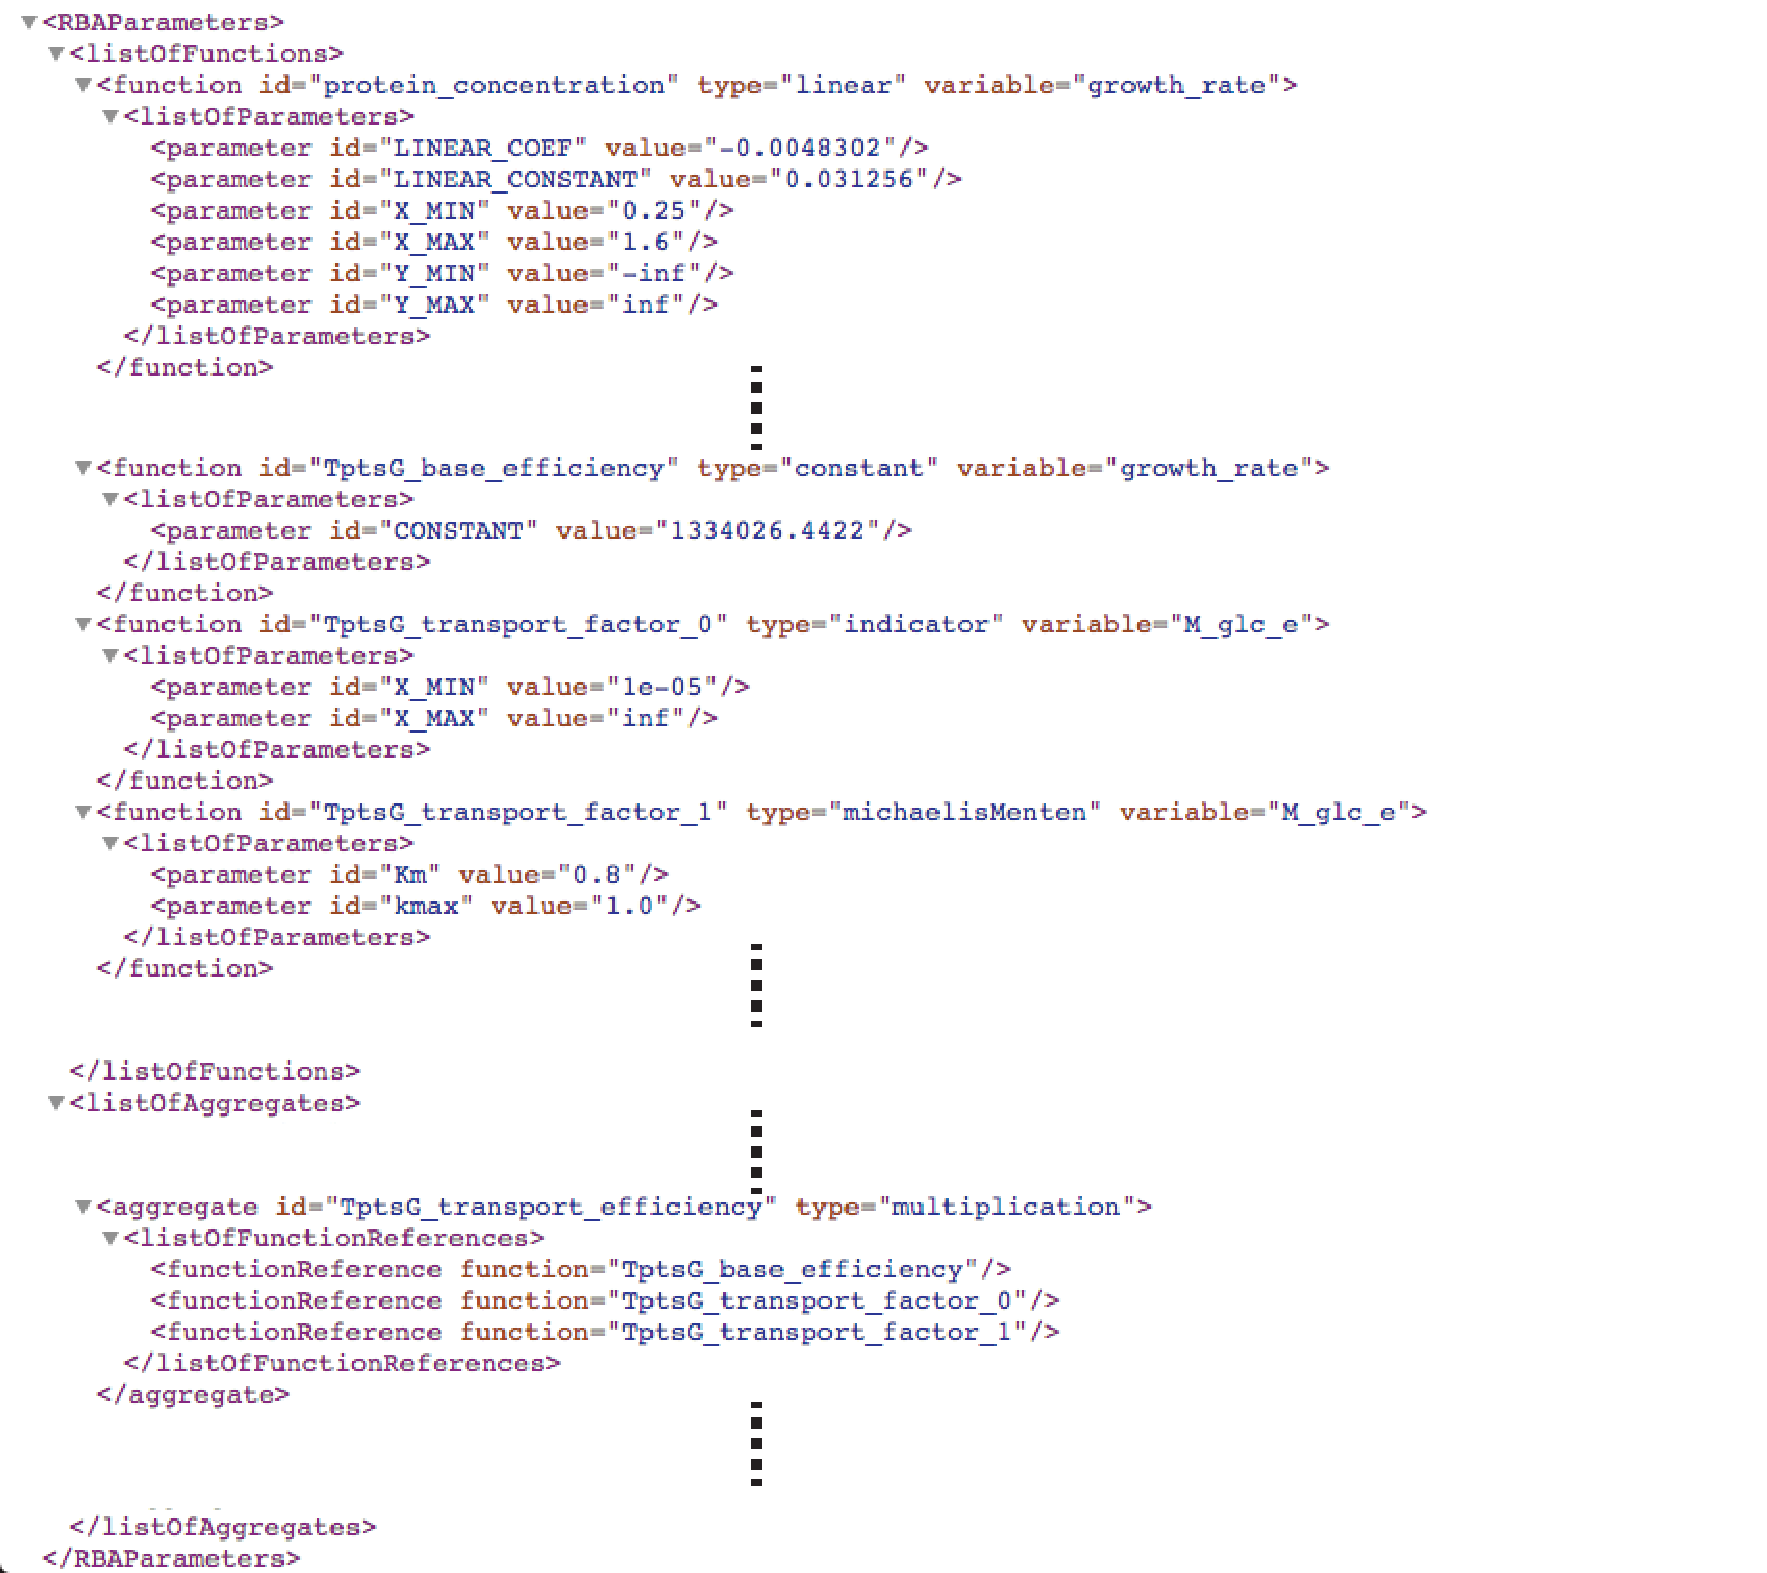
\includegraphics[scale=0.6]{figures/parameters_ex_1}
  \caption{parameters.xml from a hand-curated model for model bacteria \textit{B. subtilis}.
  Large parts of the file were removed for brevity.
  Parameters are defined either as constants, functions (e.g. linear or Michealis-Menten),
  or aggregates, representing the multiplication of functions.
  Functions can be defined in terms of growth rate (the default) or concentration
  of external metabolites.
  Aggregates may contain an arbitrary number of functions,
  and functions in an aggregate can be defined according to different variables
  (growth rate, concentration of different metabolites).}
  \label{fig:parameters_ex_1}
\end{figure}

\begin{figure}
  \centering
  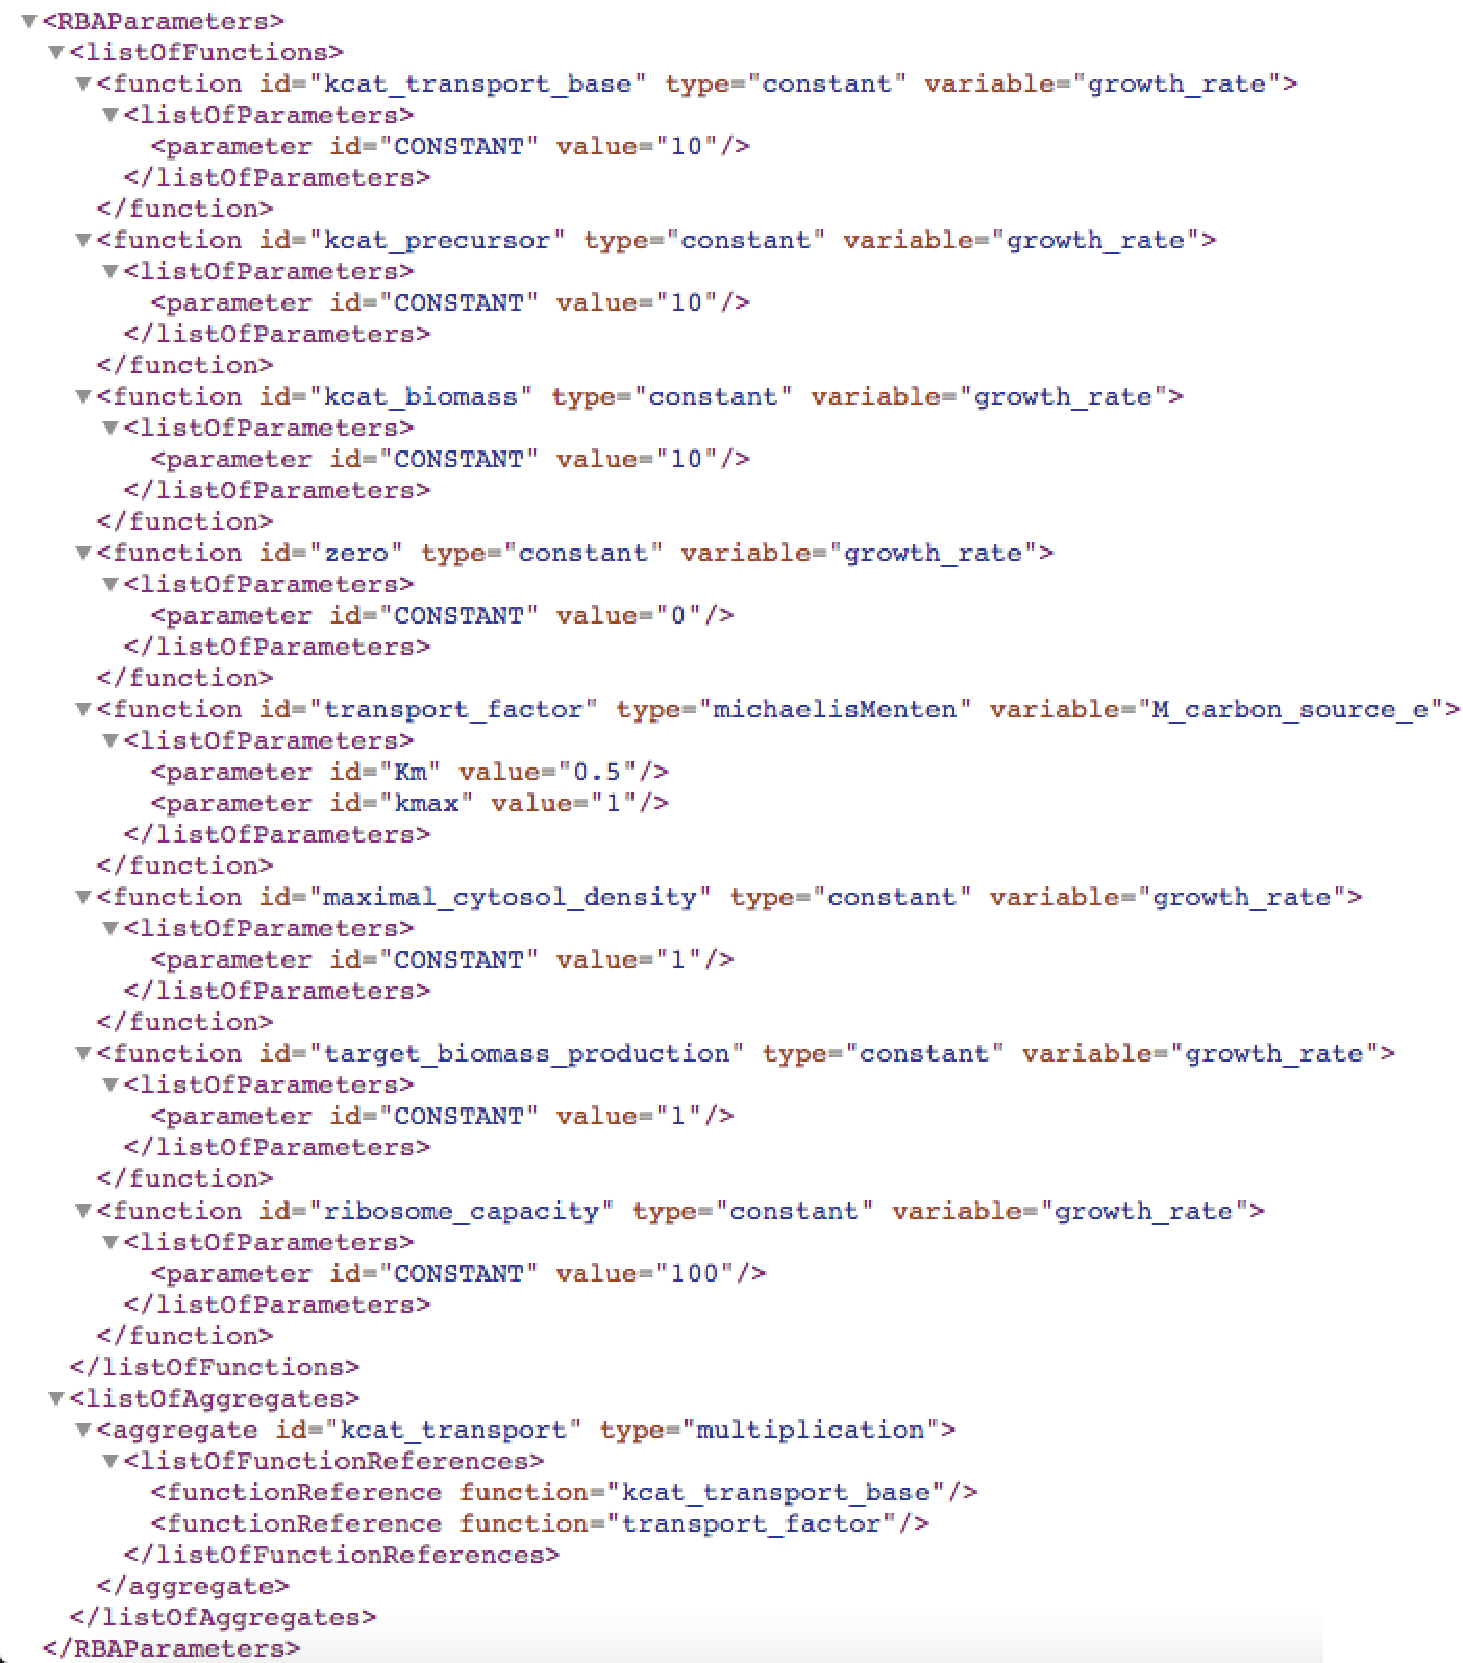
\includegraphics[scale=0.6]{figures/parameters_ex_2}
  \caption{parameters.xml from the minimal model.
  For simplicity, all parameters were defined as constants,
  except for transport terms, which adopt the traditional Michaelis-Menten.}
  \label{fig:parameters_ex_2}
\end{figure}



\end{document}
% ----------------------------------------------------------------
